\section{Introduction}\label{section introduction}


{\bf Context.} In the quite informal paper \cite{DBLP:journals/corr/PrasadZ16}, Prasad and Zuck studied resilience of a process to an adversary and they used the framework of WSTS enjoying both upward and downward monotonies to prove the decidability of a kind of resilience.
%
%{\bf MFCS 2023
%Abstract submission deadline:    	 April 24th (AoE) 
%Paper submission deadline:    	April 28th (AoE)} \\
%%
%{\bf CONCUR 2023 Abstract Registration Due 	Apr 24, 2023
%Submission Deadline 	May 2, 2023}\\
%
{\bf FSTTCS 2033  Submission deadline: July 14, 2022 AoE (firm)
Notification to authors: September 16, 2022}

trop d'hypotheses trop fortes sur les WSTS

{\bf Our contributions}
We introduce a more general definition of resilience generalising the two given in \cite{DBLP:conf/gg/Ozkan22}.
Surprinsingly, the general undecidability statements were not known neither proved.

\begin{itemize}

\item safe clos haut, bad clos par le bas: resilience = reachability d'un clos par le bas (anti-coverability)

\item safe clos haut : resilience indecidable for WSTS with strong.

\end{itemize}



Some systems are subjects at frequent intervals to accidents, attacks or changes. Think for instance of a supply chain, or an airport’s air trafic control. In such cases, a question that arises is that of whether the system can return to its normal (safe) behavior after an accident or attack [pushed it towards some kind of ‘error state’] and, if it can, whether it can perform the return in a satisfactory timeframe. In the exemple of air trafic control, an accident i.e. for instance a delay in the arrival of a plance can lead to conflicts of resolution (i.e. landing) which lead to prompting planes to remain on standby. Since their fuel quantity is limited it is hence pretty important to be able to know that trafic will return to its normal pace quickly enough. This is the resilience problem. 

Resilience is a concept of growing interest [references]. Both Okzan and Würdemann [ref] and Prasad and Zuck [ref] have started to consider [casting the problem into] the framework of Well-Structured Transition Systems. 
 
Resilience is an instance of the home space problem: let $L_1,L_2$ be two sets of states, the home space for  $L_1,L_2$ is the following question:		
	$\post^*(L_1)	\subseteq \pred^*(L_2)$


\begin{center}
	\begin{figure}
			\hspace{0.75cm}
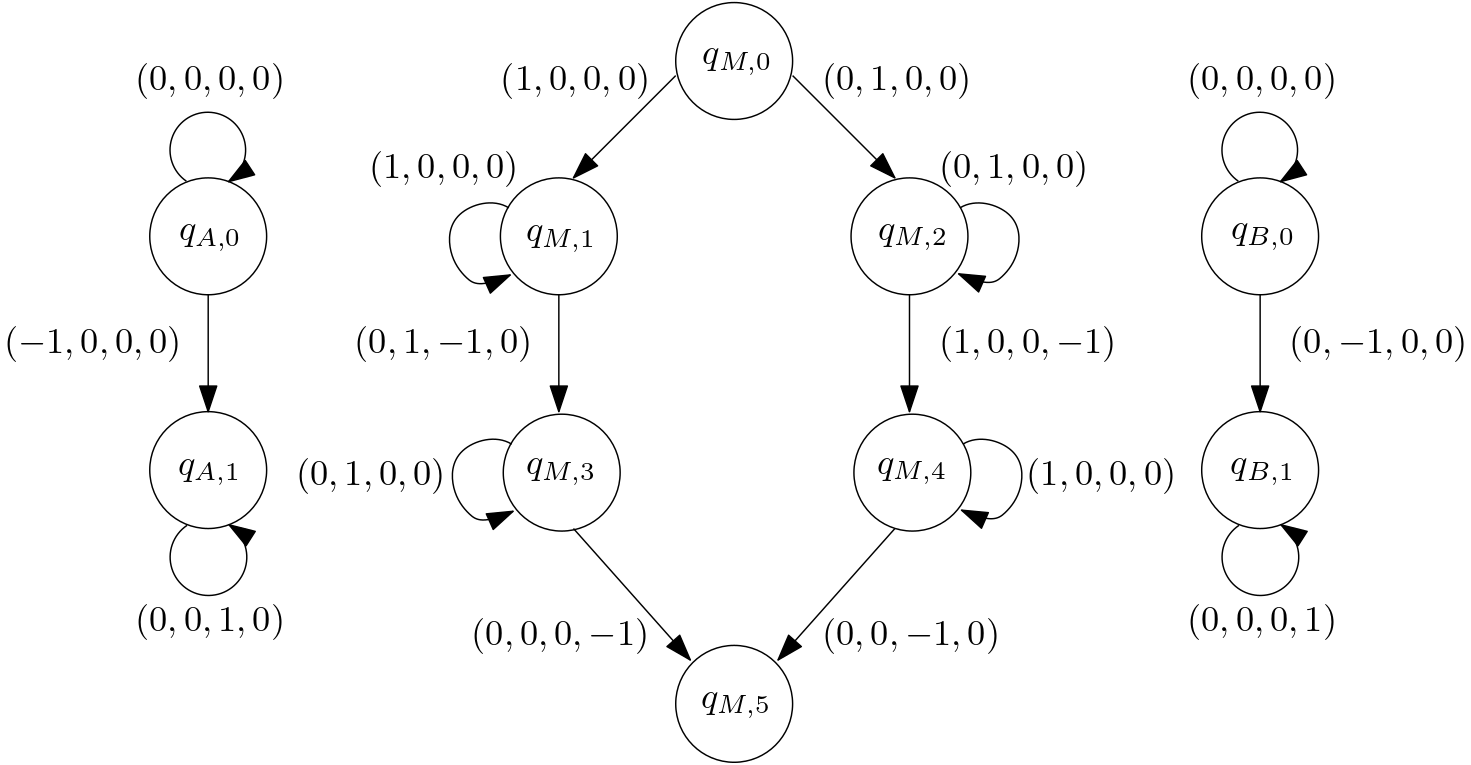
\includegraphics[width=0.85\textwidth]{FigureB}
	\caption{A channel system with three automata and four channels. Leftmost and rightmost automata represents aircrafts attempting to land and staying on stand-by in the air while they haven't received permission to land, while the middle one represent the control tower managing the aircrafts landings so that only one aircraft at a time is allowed for landing.}
					\label{air control}
	\end{figure}
\end{center}

Consider the channel system in Figure~\ref{air control}. It models a scenario in which two aircrafts wants to land in an airport at the same time. 

The automata on the left and right represents the aircrafts attempting to land, while the middle one represent the control tower. The control tower can send messages to the aircrafts using channels $c_1$ and $c_2$, and these in turn can send messages to the control tower using respectively channel $c_3$ and $c_4$. Remark channels $c_3$ and $c_4$ have a unary alphabet
in the exemple and therefore can be seen as counters. 

Safety requires that only one aircraft at a time attempt to land. The role of the control tower is to ensure this;
there are two possible choices: aircraft A waits for aircraft B to land
or vice-versa. To make its choice known to the aircrafts, the control tower will send them messages using the channels. 
We assume that the channel are
lossy \-- i.e. an arbitrary number of messages may be lost from the channels \--  but that they are still such that out of ten messages, at least one is not lost.
In this example, the safe, desirable state would be one where the aircrafts have both landed. 
Resilience here expresses that the aircrafts state will both land, while explicit resilience or $k$-resilience asks whether they will do so in at most $k$ steps. 
Explicit resilience is of interest since in general we want to ensure the safe state will
be reached in
the least amount of step possible. 
In this exemple, for instance, aircrafts cannot simply wait in the air an infinite amount of time.
With one out of ten messages guarranteed to not be lost, $40$-resilience hold in the example.

\alain{il faut mieux expliquer le modèle, le rôle des 4 canaux, des messages, remarquer que 2 canaux sont des compteurs,....}

% contrôle de trafic aérien, perturbation dans le planning → Bad (par exemple, trop d’avions qui cherchent à atterir en même temps et qui doivent être mis en stand-by au dessus de l’aéroport?) → Safe (trafic fluide à nouveau). K-résilience important car les avions peuvent pas rester indéfiniment en stand-by (re : le carburant est un réactif limitant) 



